\chapter{Metode de localizare a obiectelor}
\label{chap:localizare}

\indent\par
Detectarea unui obiect de interes într-o imagine este una dintre cele mai abordate teme din viziunea artificială. Pentru a atinge acest scop variantele sunt numeroase, toate având o caracteristică comună: dependența de trăsăturile obiectului vizat. Un exemplu practic îl reprezintă detecția fețelor în imagini: pentru ca o regiune să fie identificată drept față, aceasta trebuie să prezinte o formă aproximativ ovală, în interiorul căreia să se regăsească două zone simetrice corespunzătoare ochilor, dispuse în treimea superioară, o structură verticală alungită asociată nasului, plasată central, și o regiune orizontală sub aceasta, corespunzătoare gurii. Fiecare obiect poate fi astfel caracterizat printr-un set de trăsături distinctive geometrice, cromatice sau texturale care permit diferențierea sa de restul scenei.

În contextul lucrării de față, obiectul de interes îl reprezintă plăcuța de înmatriculare, a cărei localizare precisă constituie o secțiune critică a întregului proces. Regiunea determinată de numărul de înmatriculare poate fi localizată folosind diferite metode care pot fi clasificate în funcție de caracteristica utilizată~\cite{SOAReview}: culoare, textură, sau contur. Ultima categorie este întâlnită cel mai frecvent în aplicații și se bazează pe presupunerea că în interiorul plăcuței există schimbări de intensitate mai drastice și mai dese decât în oricare altă zonă a imaginii. Metodele bazate pe culoare au ca fundație presupunerea că există o distincție clară între culoarea numărului de înmatriculare și fundal; iar cele pe textură se folosesc de prezența caracterelor în interiorul plăcuței pentru a delimita regiunea acestuia.

\subsection{Metode bazate pe caracteristici cromatice}
\indent\par
Această categorie de metode vizează obiectele care prezintă în interiorul lor o paletă cromatică bine definită și ușor diferențiabilă de fundalul imaginii. Un exemplu clasic îl reprezintă localizarea semnelor de circulație, a căror culoare standardizată permite separarea lor de restul scenei.

Punctul de plecare al acestor metode îl constituie alegerea unui model cromatic. Un model cromatic reprezintă un model matematic abstract care descrie modul în care culorile pot fi reprezentate într-un spațiu cu mai multe dimensiuni, cel mai frecvent tridimensional. Modelul RGB (Red, Green, Blue) descrie fiecare culoare prin combinația aditivă a trei componente de bază și corespunde modului în care senzorii camerelor digitale achiziționează imaginea. Dezavantajul său major în contextul localizării este că informația despre culoare și cea despre luminozitate sunt amestecate în cele trei canale: aceeași culoare percepută își modifică semnificativ valorile RGB atunci când condițiile de iluminare se schimbă. Din acest motiv, abordările bazate pe culoare convertesc de regulă imaginea într-un model din familia HSV/HSL/HSI (Hue, Saturation, Value/Lightness/Intensity), în care nuanța (\emph{hue}) este separată de saturație și de componenta de luminozitate. Această separare conferă o anumită invarianță la variațiile de iluminare, deoarece nuanța unei culori rămâne relativ stabilă chiar și atunci când intensitatea luminii se modifică.

În cadrul sistemelor ALPR, numeroase lucrări au valorificat caracteristicile cromatice ale plăcuței pentru a o localiza~\cite{shi2005automatic},~\cite{chang2004automatic}.

Prima lucrare~\cite{shi2005automatic} tratează localizarea numerelor de înmatriculare din China, unde există un număr restrâns de combinații standardizate de culori (de exemplu, caractere albe pe fundal albastru pentru autoturisme sau caractere negre pe fundal galben pentru vehiculele de mare tonaj). Ideea de bază este că o anumită combinație culoare-fundal apare aproape exclusiv în regiunea plăcuței. Trecerea la modelul HLS rezolvă problema robusteții, dar introduce un cost de calcul prohibitiv: conversia $\text{RGB} \rightarrow \text{HLS}$ devine punctul critic, necesitând aproximativ o secundă pentru o imagine de $1024 \times 768$ pixeli. Soluția finală păstrează insensibilitatea la iluminare a modelului HLS, dar evită conversia propriu-zisă: pixelii sunt clasificați în 13 categorii definite direct în domeniul RGB, în funcție de variația luminozității. Regiunea plăcuței este apoi delimitată prin analiza histogramelor pe direcțiile verticală și orizontală și validată pe baza raportului lățime/înălțime (WHR). Sistemul atinge o rată de citire corectă de 90~\% din imagini, în mai puțin de 0,3~secunde.

\begin{figure}[h!]
  \centering
  \begin{subfigure}[b]{0.8\linewidth}
    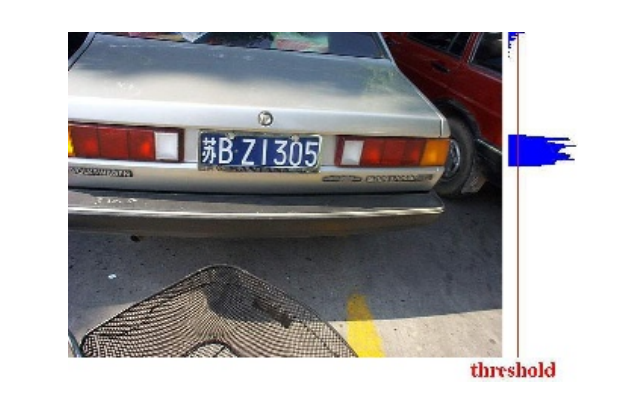
\includegraphics[width=\linewidth]{figures/shi_2005_1png.png}
    \caption{Localizarea zonei de interes generale folosind proiecții verticale}
  \end{subfigure}

  \vspace{1em}

  \begin{subfigure}[b]{0.4\linewidth}
    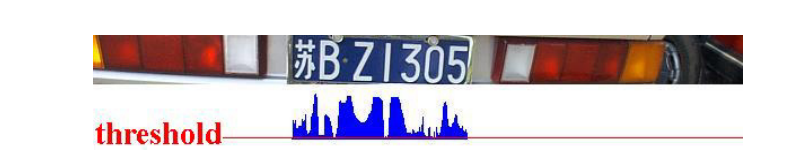
\includegraphics[width=\linewidth]{figures/shi_2005_2.png}
    \caption{Extragerea numărului de înmatriculare folosind proiecții verticale}
  \end{subfigure}
  \hfill
  \begin{subfigure}[b]{0.4\linewidth}
    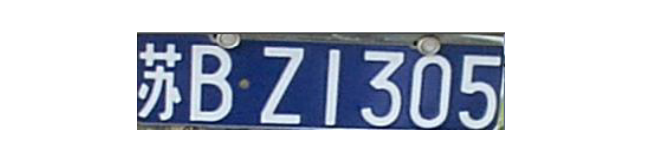
\includegraphics[width=\linewidth]{figures/shi_2005_3.png}
    \caption{Numărul de înmatriculare extras}
  \end{subfigure}
  \caption{Procesul de extracție al numărului de înmatriculare~\cite{shi2005automatic}}
\end{figure}

A doua lucrare~\cite{chang2004automatic} abordează plăcuțele din Taiwan, care utilizează patru culori distincte (alb, negru, roșu și verde). De această dată imaginea RGB este transformată efectiv în modelul HSI (Hue, Saturation, Intensity), pe baza căruia se construiește un detector de contururi cromatice. Spre deosebire de un detector de margini clasic, acesta reacționează doar la cele trei tipuri de tranziții întâlnite în interiorul plăcuței --- negru-alb, roșu-alb și verde-alb ---, ignorând restul contururilor din imagine. Pentru fiecare dintre hărțile de nuanță, saturație, intensitate și contur se calculează câte o hartă \emph{fuzzy}, ale cărei valori exprimă gradul în care fiecare pixel aparține unei plăcuțe. Cele patru hărți sunt apoi combinate printr-un agregator fuzzy în două etape, iar regiunile cu valori maxime locale și dimensiune suficientă sunt reținute drept candidați. Folosind exclusiv informația de localizare, metoda atinge o rată de succes de 97,9~\%, respectiv 93,7~\% pentru întregul sistem de recunoaștere.

Această categorie de metode prezintă atât avantaje, cât și limitări importante. Pe de o parte, atunci când contextul problemei garantează o paletă cromatică standardizată, ele oferă o acuratețe ridicată și un timp de execuție redus, datorită algoritmilor relativ simpli și ușor de optimizat. Pe de altă parte, ele nu generalizează la un spectru larg de formate, fiind dependente de un set restrâns de combinații de culori cunoscute \emph{a priori}; din acest motiv, lucrările menționate vizează țări precum China sau Taiwan, unde variațiile sunt limitate. În plus, performanța lor rămâne sensibilă la condițiile de iluminare și la degradarea cromatică a plăcuțelor reale.

\subsection{Metode bazate pe conturul obiectelor}
\indent\par
Această abordare are la bază presupunerea că în interiorul plăcuței există o densitate ridicată de linii verticale și orizontale care fac regiunea respectivă să iasă în evidență. Indiferent de abordarea ulterioară, fluxul de procesare începe întotdeauna de la transformarea imaginii în tonuri de gri. În fotografie și viziune pe calculator, o imagine în tonuri de gri este o imagine în care fiecare pixel este o nuanță de gri, unde valoarea fiecărei celule este un singur eșantion, ținând doar informația intensității. Această caracteristică a imaginilor în tonuri de gri reprezintă un factor important, deoarece în cadrul trecerilor, mai exact la marginile unui obiect apar întotdeauna diferențe mari de intensitate, cu atât mai mult în cadrul unui număr de înmatriculare unde trecerile sunt în general de la alb la negru, roșu la alb, verde la roșu, etc. Treceri bruște, clare și evidente într-o imagine convertită la alb-negru.

În~\cite{luo2009efficient} asupra imaginii convertite este aplicat operatorul Sobel pentru a extrage atât marginile verticale cât și cele orizontale. Operatorul Sobel constă în 2 kernel-uri specializate pentru detectarea liniilor convoluționate asupra întregii imagini pentru a produce un rezultat care evidențiază marginile obiectelor, trecerile bruște de la o intensitate la alta. Rezultatul intermediar generat de operatorul Sobel este binarizată folosind diferiți algoritmi de prag precum metoda histogramei, grad4 etc. Pentru o localizare robustă sunt aplicate imaginea \emph{skip} și imaginea integrală, prima având ca scop calcularea, pentru un dreptunghi de dimensiune predefinită, a distanței dintre pixelii albi și cei negri, iar imaginea integrală calculează pentru fiecare punct suma cumulativă a intensităților tuturor pixelilor aflați în regiunea superioară și stângă. Folosind această metodă, autorii au reușit să obțină o rată de localizare cu succes a numărului de înmatriculare de 99,95~\% cu un timp mediu de procesare de 47~\text{ms}.
\begin{figure}[h!]
  \centering
  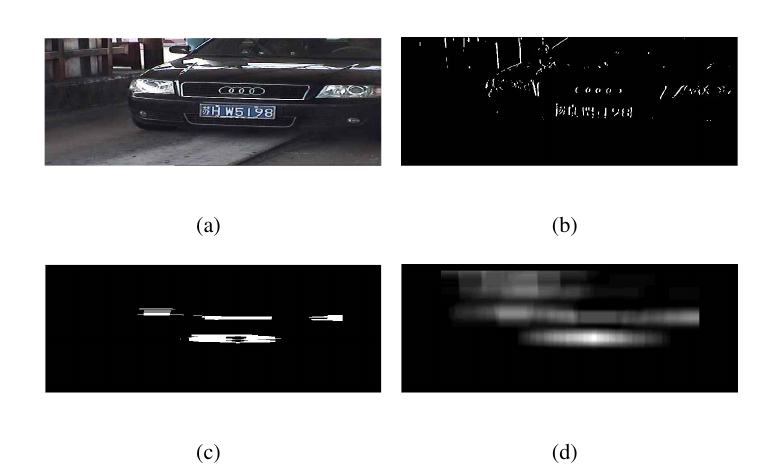
\includegraphics[width=0.6\linewidth]{figures/luo2209}
  \caption{(a) Imaginea RGB inițială, (b) Imaginea binară a marginilor, (c) Imaginea \emph{skip}, (d) Imaginea integrală~\cite{luo2009efficient}}
\end{figure}

Similar cu~\cite{luo2009efficient},~\cite{morph_operations} utilizează operatorul Sobel ca componentă primară pentru extragerea marginilor și a contururilor, totuși deosebirile apar încă din etapa de pre-procesare a imaginii (etapa de pre-procesare este formată din întreaga suită de pași aplicată imaginii înainte ca algoritmul principal de detectare a contururilor să fie rulat).~\cite{morph_operations} se folosesc de filtrul median pentru a atenua zgomotul imaginii. În viziunea pe calculator, atenuarea zgomotului presupune crearea unei funcții care capturează informațiile și tiparele imaginii lasând la o parte detaliile la scară redusă sau alte variații rapide de intensitate.

Pe lânga filtrarea mediană, pentru a asigura un rezultat robust, autorii definesc o mască de dimensiuni predefinite preluate din condiționarea problemei asupra căreia să continue cu urmatoarele etape ale procesului, respectiv operatorul Sobel, binarizarea imaginii și operația morfologică de deschidere. Aceasta din urmă constă în aplicarea consecutivă a două transformări fundamentale morfologice: eroziune și dilatare.

Operația de eroziune are rolul de a diminua obiectele din prim-plan și de a elimina structurile izolate care nu aparțin plăcuței. Aceasta presupune aplicarea unui kernel asupra întregii imagini, pixelul central fiind setat ca alb dacă toți pixelii acoperiți de kernel sunt la rândul lor albi. Operația de dilatare reprezintă opusul celei de eroziune, este formată din același algoritm, însă structura sa decizională transformă pixelul evaluat în „alb” dacă cel puțin un pixel acoperit de elementul structurant este activ.

\begin{figure}[h!]
  \centering
  \begin{subfigure}[b]{0.3\linewidth}
    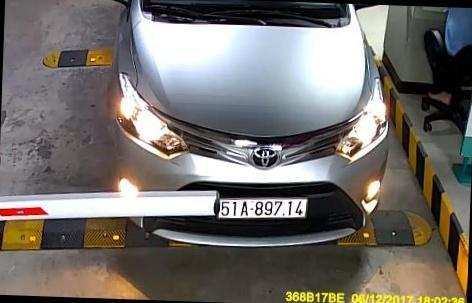
\includegraphics[width=\linewidth]{figures/input.jpg}
    \caption{Imagine de intrare}
  \end{subfigure}
  \begin{subfigure}[b]{0.3\linewidth}
    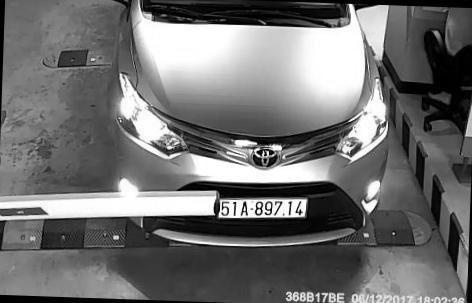
\includegraphics[width=\linewidth]{figures/greyscale.jpg}
    \caption{Imaginea în tonuri de gri}
  \end{subfigure}
  \begin{subfigure}[b]{0.3\linewidth}
    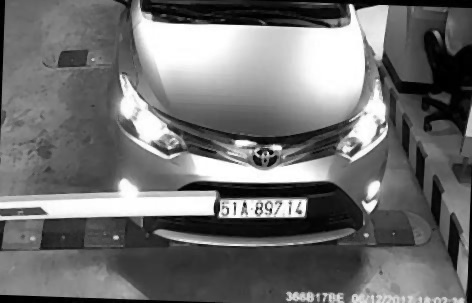
\includegraphics[width=\linewidth]{figures/median.jpg}
    \caption{Imaginea filtrată folosind filtrul median}
  \end{subfigure}
  \begin{subfigure}[b]{0.3\linewidth}
    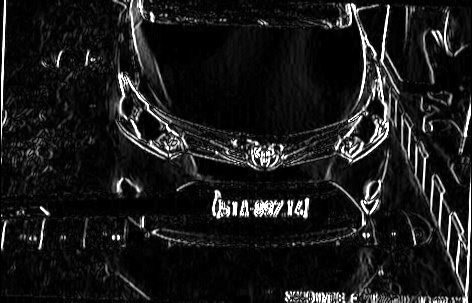
\includegraphics[width=\linewidth]{figures/sobel.jpg}
    \caption{Imaginea Sobel}
  \end{subfigure}
  \begin{subfigure}[b]{0.3\linewidth}
    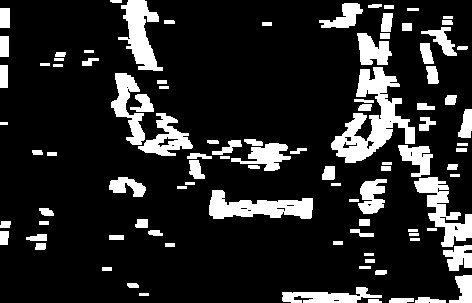
\includegraphics[width=\linewidth]{figures/open_image.jpg}
    \caption{Imaginea deschisă}
  \end{subfigure}
\end{figure}

Deși Sobel oferă rezultate bune, costul său din punct de vedere computațional a motivat autorii lucrării~\cite{VEDA} să dezvolte un nou algoritm pentru detectarea marginilor verticale. Metoda propusă omite în totalitate marginile orizontale din cadrul unei imagini, axându-se strict pe cele verticale. Această decizie a fost fundamentată pe observația că marginile orizontale pot cauza diferite elemente din compoziția mașinii precum grilajul să fie identificate în mod eronat drept numere de înmatriculare.

Fluxul de procesare propus în~\cite{VEDA} diferă față de cele menționate anterior. Inițial, asupra imaginii greyscale îî este aplicat un algoritm de binarizare cu prag adaptiv.

Acesta este urmat de ULEA (Unwanted Line Elimination Algorithm), un procedeu specializat de eliminare a artefactelor generate de către binarizare și a liniilor verticale nedorite de o lățime predefinită.

În final este aplicat VEDA, propus ca înlocuitor al operatorului Sobel de către autori. Această metodă constă în convoluționarea unui kernel de $2\times4$ asupra întregii imagini și o structură decizională care selectează un pixel ca fiind activ sau inactiv pe baza unor reguli logice în locul operațiilor clasice de convoluție.

Prin renunțarea la procesarea liniilor orizontale și optimizarea mecanismului de detecție, algoritmul propus are o viteză medie de rulare de 15~\text{ms}, o îmbunătățire semnificativă în comparație cu operatorul Sobel, care atinge o viteză medie de 130~\text{ms}.

\begin{figure}[h!]
  \centering
  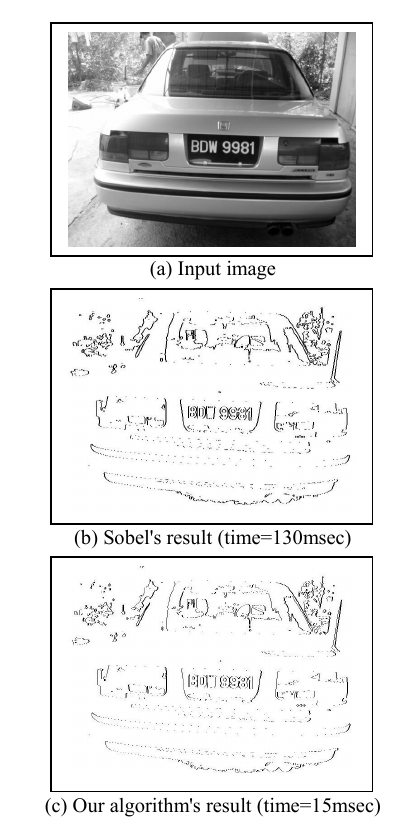
\includegraphics[width=0.3\linewidth]{figures/veda.png}
  \caption{Comparație între rezultatele generate de Sobel și VEDA~\cite{VEDA}}
\end{figure}

Datorită faptului că~\cite{luo2009efficient},~\cite{morph_operations},~\cite{VEDA} folosesc drept componentă principală operatorul Sobel, respectiv VEDA, aceste abordări sunt capabile să localizeze plăcuțe conținând numere de înmatriculare aflate în imagine la o înclinație de până la 15~\textdegree. Pentru a combate acest lucru, în~\cite{HoughTransformation} este folosit operatorul Hough drept selector principal.

Spre deosebire de operatorii de gradient (Sobel sau VEDA), care se bazează pe analiza locală a pixelilor, transformarea Hough reprezintă o tehnică de extracție a caracteristicilor utilizată pentru a identifica forme geometrice prin procesul de votare într-un spațiu al parametrilor. În contextul localizării numerelor de înmatriculare, aceasta este utilizată preponderent pentru detecția liniilor drepte care definesc conturul dreptunghiular al plăcuței.

Principiul fundamental constă în maparea fiecărui punct de margine $(x, y)$ din spațiul imaginii în spațiul polar $(\rho, \theta)$, utilizând ecuația:
$$\rho = x \cos(\theta) + y \sin(\theta)$$unde $\rho$ reprezintă distanța perpendiculară de la origine la dreaptă, iar $\theta$ este unghiul dintre axa $x$ și această perpendiculară.

Implementarea transformatii Hough în detrimentul implementării operatorului Sobel sau VEDA aduce anumite avantaje din punct de vedere al fiabilității sistemului, acesta fiind capabil sa localizeze în mod corect plăcuțe de înmatriculare înclinate la 30~\textdegree comparat cu 15~\textdegree. De asemenea, transformarea Hough nu este atât de sensibilă la variațiile de intensitate ale imaginii, astfel că o imagine de calitate nu este imperios necesară.

Totuși, performanța sporită vine cu un cost de complexitate computațională ridicat. Deoarece procesul de votare trebuie efectuat pentru fiecare pixel de margine și pentru o gamă largă de unghiuri, consumul de memorie (pentru matricea acumulator) și timpul de procesare sunt semnificativ mai mari față de un operator de convoluție simplu precum Sobel. Din acest motiv, în sistemele de timp real, transformarea Hough este adesea aplicată pe o regiune de interes (ROI) restrânsă sau este precedată de o etapă de binarizare agresivă pentru a reduce numărul de pixeli procesați.

\subsection{Metode bazate pe textura obiectelor}
\indent\par
Metodele bazate pe textură pornesc de la presupunerea că în interiorul numerelor de înmatriculare prezența caracterelor oferă o textură specifică și ușor diferențiabilă în comparație cu fundalul/ restul elementelor prezente în imagine.

În literatura de specialitate, există multiple abordări ale acestei categorii de metode,~\cite{bremananth2005robust},~\cite{anagnostopoulos2006license}, care se diferențiază prin modul în care este descrisă textura caracterelor și prin tehnica folosită pentru a evidenția regiunile cu densitate ridicată de tranziții.

În~\cite{bremananth2005robust} autorii aleg drept caracteristică definitorie a texturii densitatea de linii verticale prezente în cadrul numărului de înmatriculare. Aceștia propun un sistem al cărui prim pas este scăderea cromatică (\emph{color subtraction}), un algoritm ce primește ca parametri de intrare imaginea achiziționată anterior și o listă de elemente dintr-unul dintre modelele cromatice posibile; acest algoritm va păstra activi din imagine doar pixelii ale căror valori apar în lista primită drept parametru de intrare, iar pe restul îi va dezactiva. Următorul pas este aplicarea operatorului Sobel pentru a evidenția liniile verticale. În continuare va fi construită o hartă de densitate ponderată (\emph{weight-based density map}) folosind următorul algoritm de asignare a greutăților, în care creșterea, respectiv descreșterea unei greutăți asignate este direct proporțională:
\begin{align}
  W_{t_{\text{decr}}} &\propto (i - p) \\
  W_{t_{\text{decr}}} &\propto \gamma \\
  W_{t_{\text{decr}}} &= \partial\,\gamma\,(p - i) \\
  W_t &= \sum_{i=0}^{n} t_w \left( W_t + (px_i)\gamma + (1 - px_i)\big(\partial\gamma(p - i)\big) \right) \\
  t_w &= \frac{W_t - |W_t|}{-2W_t}\,\beta + \frac{W_t + |W_t|}{2W_t}
\end{align}
unde $\partial$ este constanta de decădere (\emph{decay constant}), $\gamma$ este factorul de incrementare a greutății, $\beta$ greutatea inițială, $n$ numărul de puncte de coordonate, $i$ coordonata muchiei curente, $p$ coordonata muchiei anterioare, iar $W_t$ valoarea greutății.

După finalizarea construcției hărții de densitate putem identifica posibilele regiuni în care apare un număr de înmatriculare.

Spre deosebire de~\cite{bremananth2005robust}, care descrie textura prin densitatea liniilor verticale, în~\cite{anagnostopoulos2006license} autorii pornesc de la ideea că plăcuța poate fi privită ca o regiune în care textura imaginii prezintă o „neregularitate'' locală pronunțată, mai exact treceri bruște și dese între caracterele întunecate și fundalul deschis. Pentru a evidenția aceste zone, ei propun o tehnică de segmentare adaptivă numită SCW (Sliding Concentric Windows), care nu măsoară direct contururile, ci variația statistică a intensităților dintr-o vecinătate.

Metoda se bazează pe utilizarea a două ferestre dreptunghiulare concentrice, una interioară $A$ de dimensiune $(2X_1) \times (2Y_1)$ și una exterioară $B$ de dimensiune $(2X_2) \times (2Y_2)$, care parcurg împreună întreaga imagine, pixel cu pixel, pornind din colțul stânga-sus. Pentru fiecare poziție se calculează în cele două ferestre câte o măsură statistică $M$ (media sau deviația standard a intensităților), iar pixelul central este clasificat în funcție de raportul dintre cele două măsuri:
$$I_{\text{AND}}(x, y) = \begin{cases} 0, & \text{dacă } \dfrac{M_B}{M_A} \leq T \\[2mm] 1, & \text{dacă } \dfrac{M_B}{M_A} > T \end{cases}$$unde $T$ este un prag stabilit experimental. Atunci când raportul depășește pragul, vecinătatea pixelului prezintă o variație texturală suficient de mare pentru ca acesta să fie considerat parte a unei regiuni de interes. Parametrii $X_1, X_2, Y_1, Y_2$ se aleg astfel încât raportul de aspect al ferestrelor să fie apropiat de cel al obiectelor căutate (caracterele plăcuței).

Imaginea binară $I_{\text{AND}}$ obținută prin SCW este apoi combinată cu imaginea originală printr-o operație logică ȘI, rezultatul fiind binarizat cu ajutorul metodei de prag adaptiv Sauvola, în care pragul fiecărui pixel depinde de media și deviația standard locale dintr-o fereastră de dimensiune $b \times b$:
$$T(x, y) = m(x, y)\left[1 + k\left(\frac{\sigma(x, y)}{R} - 1\right)\right]$$Asupra imaginii binarizate se aplică o analiză a componentelor conexe (CCA), iar obiectele rezultate sunt filtrate pe baza unor criterii geometrice: raportul de aspect, orientarea (sub $35~\textdegree$) și numărul Euler. Acesta din urmă, definit ca diferența dintre numărul de obiecte și numărul de „găuri'' interioare, este folosit pe baza observației că o plăcuță validă conține cel puțin patru caractere, deci minimum trei goluri ($E > 3$); regiunile care nu îndeplinesc aceste condiții sunt eliminate. Pentru a trata și plăcuțele cu fundal închis și caractere deschise, dacă nicio regiune candidată nu este găsită, imaginea este inversată și întregul proces reia.

Etapa de localizare este urmată de segmentarea caracterelor, realizată tot prin SCW aplicat regiunii decupate, și de recunoașterea propriu-zisă cu o rețea neuronală probabilistică (PNN) cu topologia $108\text{-}180\text{-}36$. Testat pe un set de 1334 de imagini din scene naturale, cu fundaluri și condiții de iluminare variate, sistemul a segmentat corect plăcuța în 96,5~\% din cazuri, recunoașterea întregii plăcuțe atingând 89,1~\%, respectiv o rată globală de succes de 86~\%.
